\CQUsection{模型设计}

\CQUsubsection{研究方法总体框架}
本文面向颅内动脉瘤智能分析任务，构建了由病灶分割与破裂风险评估组成的两阶段研究框架。该框架遵循“病灶定位—特征生成—风险判别”的基本逻辑：首先利用三维分割网络对 CTA 体数据中的疑似动脉瘤区域进行体素级识别，获得病灶概率分布与空间掩膜；随后基于分割结果与病例层面的临床、形态及影像表型信息构建统一的特征表示，并输入风险预测模型完成患者级破裂概率估计。该流程兼顾了医学影像任务中病灶分割与辅助临床决策的双重需求。

从形式化角度看，设单例 CTA 体数据记为 $X\in\mathbb{R}^{D\times H\times W}$，其对应分割标注为 $Y^{(s)}\in\{0,1\}^{D\times H\times W}$，病例级风险标签为 $y^{(r)}\in\{0,1\}$。本文方法可形式化表示为
\begin{align}
P &= f_{\theta}(X),\\
\hat{M} &= \mathcal{T}(P;\tau_s),\\
z &= \phi(X,\hat{M},c),\\
\hat{p} &= g_{\omega}(z),
\end{align}
其中，$f_{\theta}(\cdot)$ 表示分割网络，$P\in[0,1]^{D\times H\times W}$ 为体素级概率图，$\mathcal{T}(\cdot)$ 为基于阈值 $\tau_s$ 的二值化映射，$c$ 表示病例层面的临床及影像表型变量，$\phi(\cdot)$ 表示多源特征构造过程，$g_{\omega}(\cdot)$ 为风险预测模型，$\hat{p}\in[0,1]$ 为动脉瘤破裂概率估计。由此，本文实际上将像素级结构识别与样本级风险判别纳入统一分析链条，在保证解剖定位能力的同时增强风险建模的结构依据。

从任务之间的关联看，分割模块与风险预测模块并非相互独立的两个流程，而是具有明确的信息传递关系。分割模块输出的掩膜可继续用于风险模型的特征生成部分，使风险模型得到有效数据来预案，而非整幅影像中的无关背景，同时也能实现有模型解耦。若将病例级风险判别写作条件概率建模问题，则可进一步表示为
\begin{equation}
\hat{p}=\Pr\left(y^{(r)}=1\mid X,\hat{M},c\right),
\end{equation}
其中 $\hat{M}$ 提供病灶位置和形态先验，$c$ 提供病例层面的临床与表型信息。在风险预测流程中，风险预测并非仅依赖原始影像或单一临床变量，而是建立在影像结构信息与病例属性共同约束之上。

在整体设计上，本文遵循三个原则。第一，分割阶段应优先保证对小体积病灶的敏感性，以降低漏检对后续分析造成的影响；第二，特征表示阶段应尽量保持不同来源变量的统一表达，使连续变量、离散变量和分割衍生变量能够在同一隐空间内比较和交互；第三，风险判别阶段应避免仅依赖线性叠加，而应建模变量之间的条件依赖关系。上述原则共同构成本文方法设计的总体依据。

进一步地，本文将两阶段任务理解为具有条件依赖关系的分层建模问题。分割阶段提供对潜在病灶区域的空间估计，风险预测阶段则在该空间估计的约束下完成病例级判别。若以 $M$ 表示真实但不可直接观测的病灶结构变量，则风险预测可视为对如下后验概率的近似：
\begin{equation}
\Pr(y^{(r)}=1\mid X,c)=\int \Pr(y^{(r)}=1\mid M,c)\Pr(M\mid X)dM.
\end{equation}
由于真实结构变量 $M$ 只能通过人工标注或模型估计获得，本文采用分割网络输出的概率图 $P$ 与二值掩膜 $\hat{M}$ 作为其可计算近似。该表达说明，分割模块的意义不仅在于获得可视化结果，还在于为下游风险建模提供对病灶空间位置和形态属性的结构性约束。

为降低不同任务目标之间的混淆，本文未将分割标签与风险标签直接合并为单一目标，而是采用阶段化训练与统一评估的方式。该策略能够分别考察体素级结构识别能力和病例级风险判别能力，使各模块的误差来源更容易被分析。同时，分割输出所形成的形态特征和空间先验又可进入风险模型，从而保持两类任务之间的信息关联。

\CQUsubsection{分割任务的理论基础与建模动机}

颅内动脉瘤在 CTA 图像中通常表现为体积小、边界复杂且与邻近血管相互黏连的异常膨出区域，这使得分割任务面临明显的小目标、强背景干扰和类别不平衡等问题。

在这种情况下，单纯依靠局部卷积感受野容易出现两方面不足：浅层特征虽能保留较多空间细节，但语义判别能力较弱；而深层特征虽有较强的抽象表达能力，但经过多次下采样后，病灶的边界细节又容易丢失。U-Net 类编码器-解码器结构通过跳跃连接较好地平衡了这两类矛盾，因此成为三维医学图像分割的常用基础框架。

然而，标准 U-Net 在面对复杂血管背景时，仍会引入较多与病灶无关的高响应区域。有鉴于此，本文在网络主干中加入了注意力门控机制，用于抑制无关背景特征通过跳跃连接的传播；同时在瓶颈层引入多尺度上下文增强模块和方向敏感注意力，以更好地捕捉病灶的尺度变化、形态不规则性以及复杂的空间走向。这种设计的核心考虑在于：病灶分割不能仅依赖局部灰度差异，而是需要综合局部边界、邻域血管拓扑关系以及多尺度上下文信息进行联合判断。


\CQUsubsection{动脉瘤分割模块设计}
\CQUsubsubsection{输入表示与数据采样机制}
由于 CTA 体数据具有高维、稀疏和病例间差异较大的特点，本文首先对输入体数据进行统一空间归一化与强度规范化，以减弱扫描条件、体素间距与成像范围差异对模型学习带来的干扰。对于归一化后的三维影像，训练阶段采用基于局部补丁的学习方式，以在有限显存约束下维持足够的空间上下文范围；验证与测试阶段则通过覆盖式滑窗实现覆盖整个数据的推理，保证输出结果的完整性与连续性，减小patch边缘的影响。

动脉瘤区域在整个 CTA 体积数据中通常只占很小的比例。如果采用完全均匀的采样策略，训练过程中模型容易被大量背景区域主导，导致对前景病灶的召回率不足。为此，本文采用了一种兼顾前景强化与背景约束的补丁采样机制：在构造训练样本时，适当提高病灶及其邻域补丁的出现概率，以增强网络对少数类（病灶）的感知能力；同时保留一定比例的背景补丁，帮助模型维持对正常解剖结构的判别边界。该策略本质上是一种面向类别不平衡场景的数据分布重加权方法，能够有效提升模型对小体积病灶的学习效率。设从整例体数据中抽取补丁 $x_p$ 的采样分布为 $\pi(x_p)$，则经验风险表示为
\begin{equation}
\widehat{R}(\theta)=\frac{1}{B}\sum_{b=1}^{B}\mathcal{L}\left(f_{\theta}(x_{p_b}),y_{p_b}\right),\quad x_{p_b}\sim\pi(x_p),
\end{equation}
其中 $B$ 为批量大小。当前景邻域补丁的采样概率被适度提高时，训练过程中的梯度估计将包含更多与病灶相关的局部模式，从而缓解由背景样本占比过高导致的优化偏置。与此同时，保留背景补丁可避免模型仅学习前景邻域的局部统计特征，进而维持对正常血管和非目标组织的辨别能力。

在补丁学习框架下，局部样本的空间覆盖范围也会影响模型可获得的上下文信息。若补丁尺寸过小，模型虽然能够获得更多前景样本，但可能无法完整观察动脉瘤与载瘤血管之间的空间关系；若补丁尺寸过大，则单批次中前景体素占比进一步降低，且训练计算负担增加。因此，补丁采样需要在局部细节、上下文范围与类别平衡之间取得折中。该折中可理解为对训练分布 $\pi(x_p)$ 的约束优化：
\begin{equation}
\pi^{\ast}=\arg\min_{\pi}\left|\mathbb{E}_{x_p\sim\pi}[r(x_p)]-r_0\right|+\lambda_c\mathcal{C}(x_p),
\end{equation}
其中 $r(x_p)$ 表示补丁中的前景比例，$r_0$ 表示期望的前景可见程度，$\mathcal{C}(x_p)$ 表示上下文不足或计算代价带来的约束项，$\lambda_c$ 为权衡系数。该表达并非要求严格求解采样分布，而是说明补丁构造应兼顾病灶可见性与上下文完整性。

\CQUsubsubsection{三维 Attention U-Net 主干结构}
分割主干采用三维 Attention U-Net。编码器由多层三维卷积块和逐级下采样操作构成，用于提取从低层纹理到高层语义的分层特征；解码器则通过上采样和特征融合逐步恢复空间分辨率，实现精细的体素级预测。设第 $l$ 层编码器特征为 $E_l$，解码器特征为 $D_l$，则主干网络可抽象为下式：
\begin{align}
E_l &= \mathcal{E}_l(E_{l-1}), \quad l=1,2,\ldots,L,\\
B &= \mathcal{B}(E_L),\\
D_l &= \mathcal{D}_l(D_{l+1},\widetilde{E}_l), \quad l=L-1,\ldots,1,
\end{align}
其中，$\mathcal{E}_l(\cdot)$ 表示第 $l$ 层编码映射，$\mathcal{B}(\cdot)$ 表示瓶颈层特征变换，$\mathcal{D}_l(\cdot)$ 表示第 $l$ 层解码映射，$\widetilde{E}_l$ 为经注意力筛选后的跳跃连接特征。通过这种由粗到细的层级重建过程，网络能够同时利用深层全局语义信息与浅层边界细节信息，从而提高病灶轮廓恢复能力。

从特征尺度角度看，编码器逐级压缩空间分辨率并扩大有效感受野，使高层特征能够表达病灶与邻近血管之间的上下文关系；解码器则逐级恢复分辨率，使预测结果重新对齐至原始体素网格。若记第 $l$ 层特征的空间尺度为 $(D_l,H_l,W_l)$、通道数为 $C_l$，则 $E_l\in\mathbb{R}^{C_l\times D_l\times H_l\times W_l}$。随着层级加深，$(D_l,H_l,W_l)$ 逐渐减小而 $C_l$ 通常增加，模型由此在空间精度与语义抽象之间形成层次化表示。跳跃连接的作用在于将浅层空间细节重新注入解码路径，避免小病灶在连续下采样过程中被过度平滑。

更具体地，三维卷积块可被视为在局部邻域内对体素上下文进行加权聚合。设输入特征为 $U\in\mathbb{R}^{C_{in}\times D\times H\times W}$，卷积核为 $K\in\mathbb{R}^{C_{out}\times C_{in}\times r_d\times r_h\times r_w}$，则输出特征在位置 $(i,j,k)$ 的第 $c$ 个通道可写为
\begin{equation}
V_{c,i,j,k}=\sigma\left(\sum_{c'=1}^{C_{in}}\sum_{a,b,m}K_{c,c',a,b,m}U_{c',i+a,j+b,k+m}+b_c\right),
\end{equation}
其中 $\sigma(\cdot)$ 表示非线性激活函数。该形式说明，网络通过层层局部聚合逐步扩大感受野，并在通道维度上形成多级语义表示。对于动脉瘤这类小目标结构，浅层卷积更关注边缘和局部灰度变化，深层卷积则更关注病灶与周围血管之间的空间关系，二者通过跳跃连接实现互补。

此外，编码器与解码器之间的特征融合并非简单的尺度恢复过程，而是一个语义信息与定位信息重新对齐的过程。若将上采样后的解码特征记为 $U_l$，跳跃连接特征记为 $\widetilde{E}_l$，则融合操作概括为
\begin{equation}
D_l=\rho_l\left(\operatorname{Concat}(U_l,\widetilde{E}_l)\right),
\end{equation}
其中 $\rho_l(\cdot)$ 表示卷积融合映射。该操作使网络能够利用深层语义判断目标类别，同时利用浅层细节修正边界位置，从而提升小体积分割目标的空间一致性。

\begin{figure}[htbp]
    \centering
    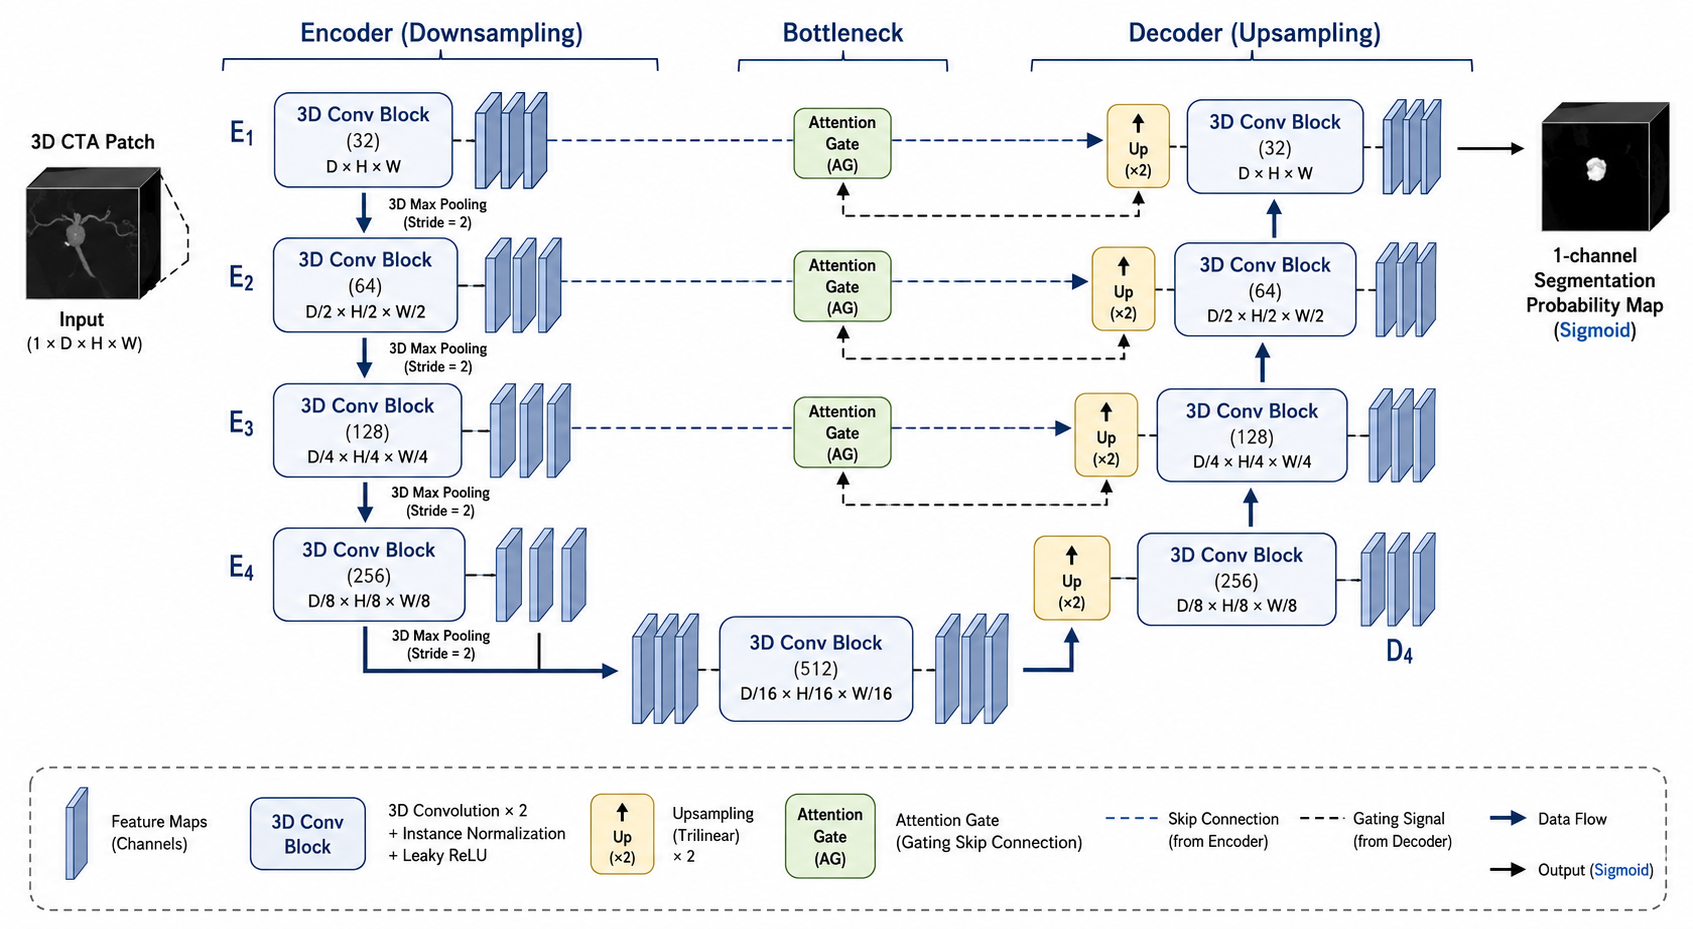
\includegraphics[width=0.95\textwidth]{figure/split_arch.png}
    \caption{三维 Attention U-Net 分割模型结构}
    \label{fig:split_arch}
\end{figure}

\CQUsubsubsection{注意力门控跳跃连接机制}
在传统 U-Net 中，编码器特征通常直接与对应尺度的解码器特征拼接。这种做法虽然有助于恢复空间分辨率，但也可能将大量背景响应一并引入解码过程，尤其是在血管、骨性结构及噪声干扰较强的 CTA 场景下更为明显。为缓解这一问题，本文在跳跃连接中采用注意力门控机制，使网络能够依据当前解码语义状态自适应选择更具判别力的编码特征。

设同尺度跳跃特征为 $s$，来自解码端的门控信号为 $g$，则注意力门控为
\begin{align}
q &= \mathrm{ReLU}(W_s s + W_g g + b),\\
a &= \sigma(\psi(q)),\\
\hat{s} &= a \odot s,
\end{align}
其中，$W_s$ 与 $W_g$ 为线性投影，$\psi(\cdot)$ 为通道压缩映射，$\sigma(\cdot)$ 为 Sigmoid 函数，$a$ 为取值于 $[0,1]$ 的注意力权重图，$\odot$ 表示逐元素乘法。该结构的本质是在跳跃连接处引入条件选择机制：当某些空间位置与当前解码语义更加一致时，对应权重被放大；反之，则被抑制。由此可降低无关背景特征对后续重建的干扰，提高分割结果的病灶聚焦能力。

\CQUsubsubsection{ASPP 多尺度上下文增强模块}
动脉瘤的空间形态在不同病例之间可能表现出明显差异，既包括局部球囊样膨出，也包括与载瘤血管边界过渡不清的复杂结构。因此，仅依赖固定尺度卷积核难以充分描述病灶及其邻近血管的多尺度上下文关系。为增强瓶颈层对不同尺度模式的响应能力，本文引入三维 ASPP 模块，通过多分支空洞卷积并行提取不同感受野下的上下文特征。

设瓶颈输入特征为 $X_b$，空洞率集合为 $\{d_1,d_2,\ldots,d_K\}$，则 ASPP 输出可表示为
\begin{equation}
Y_{\mathrm{ASPP}} = \phi\Bigl(\operatorname{Concat}\bigl[\mathcal{F}_{d_1}(X_b),\mathcal{F}_{d_2}(X_b),\ldots,\mathcal{F}_{d_K}(X_b)\bigr]\Bigr),
\end{equation}
其中，$\mathcal{F}_{d_k}(\cdot)$ 表示膨胀率为 $d_k$ 的三维空洞卷积分支，$\operatorname{Concat}[\cdot]$ 表示通道维拼接，$\phi(\cdot)$ 表示后续的线性融合与非线性映射。通过在同一层级聚合不同感受野的信息，模型能够更有效地刻画病灶本体、载瘤血管及局部背景之间的关系，从而增强对复杂形态病灶的识别鲁棒性。

\CQUsubsubsection{三维坐标注意力模块}
在多尺度上下文建模基础上，本文进一步引入三维坐标注意力模块，以增强网络对方向性位置信息的编码能力。与仅基于通道重加权的注意力形式不同，坐标注意力通过沿不同空间轴汇聚上下文信息，在保留位置依赖关系的同时生成方向敏感权重，因此更适合捕捉血管结构细长、走向复杂的空间特征。

设输入特征为 $X\in\mathbb{R}^{C\times D\times H\times W}$，则沿深度、高度与宽度方向的上下文聚合可分别表示为
\begin{equation}
Z_d=\operatorname{AvgPool}_{H,W}(X),\quad
Z_h=\operatorname{AvgPool}_{D,W}(X),\quad
Z_w=\operatorname{AvgPool}_{D,H}(X).
\end{equation}
三路聚合特征经共享映射与分支解码后得到三个方向注意力图 $A_d$、$A_h$ 与 $A_w$，最终输出为
\begin{equation}
Y_{\mathrm{CA}} = X \odot A_d \odot A_h \odot A_w.
\end{equation}
该模块通过显式建模空间方向依赖关系，使网络能够在保留通道语义的同时强化对关键位置的响应，有利于提升小病灶边界及空间走向敏感结构的识别精度。

\begin{figure}[htbp]
    \centering
    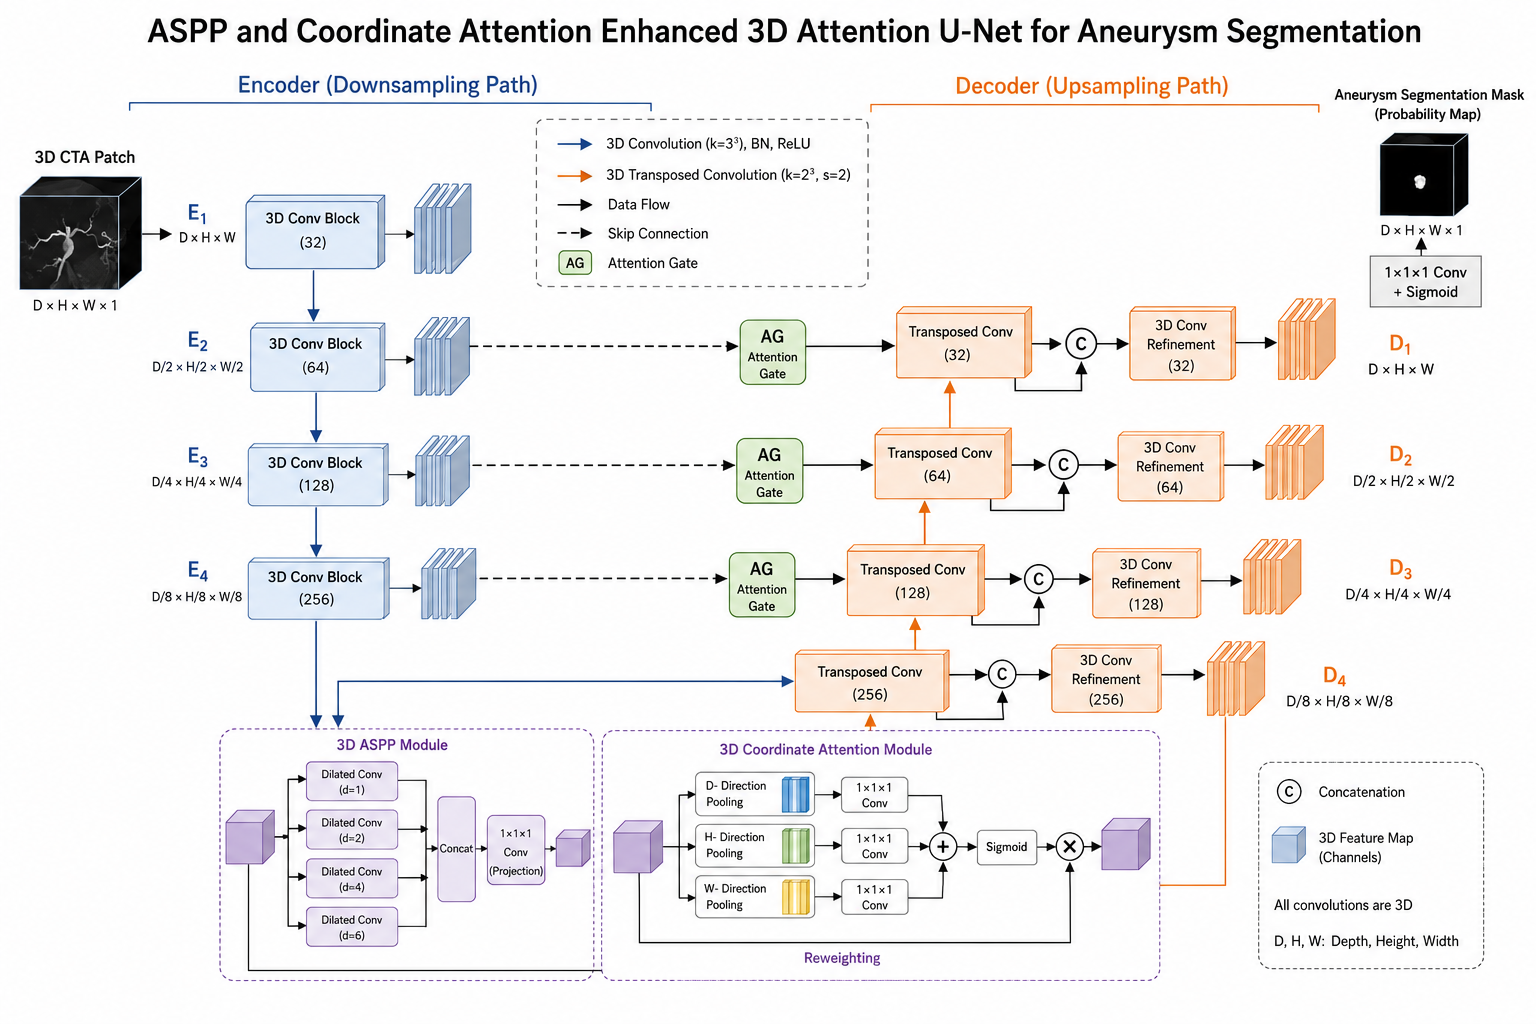
\includegraphics[width=0.95\textwidth]{figure/opt_split_arch.png}
    \caption{融合 ASPP 与三维坐标注意力的增强分割模型结构}
    \label{fig:opt_split_arch}
\end{figure}

\CQUsubsubsection{输出映射与整例重建}
在解码器末端，网络通过 $1\times1\times1$ 卷积将高分辨率特征映射到单通道对数几率空间，并经 Sigmoid 函数获得体素级前景概率图：
\begin{equation}
P_{i,j,k}=\sigma\bigl(h_{i,j,k}\bigr),
\end{equation}
其中，$h_{i,j,k}$ 表示位置 $(i,j,k)$ 处的输出 logit，$P_{i,j,k}$ 表示对应体素属于动脉瘤前景的概率。基于给定阈值 $\tau_s$，可得到二值掩膜
\begin{equation}
\hat{M}_{i,j,k}=\mathbb{I}(P_{i,j,k}\geq \tau_s),
\end{equation}
其中，$\mathbb{I}(\cdot)$ 为示性函数。

在整例推理阶段，由于输入体积较大，本文采用滑窗方式对局部补丁逐块预测，并将各窗口输出重新映射回原空间。对于重叠区域，可通过平均融合或中心区域优先策略进行整合，以减弱窗口边界效应。由此获得的整例概率图与二值分割结果，不仅可用于病灶可视化，也可进一步提取体积、尺寸及形态相关表型，为风险预测阶段提供结构性输入依据。

基于二值掩膜可计算一组具有解剖含义的形态特征。设单个体素的物理体积为 $v_{\mathrm{voxel}}$，预测前景体素集合为 $\Omega_{\hat{M}}$，则病灶体积表示为
\begin{equation}
V_{\mathrm{lesion}}=v_{\mathrm{voxel}}\sum_{(i,j,k)}\hat{M}_{i,j,k}.
\end{equation}
若进一步估计病灶表面积 $S_{\mathrm{lesion}}$，则可构造球形度等形态描述量，例如
\begin{equation}
\mathrm{Sphericity}=\frac{\pi^{1/3}(6V_{\mathrm{lesion}})^{2/3}}{S_{\mathrm{lesion}}}.
\end{equation}
该类特征能够从几何角度描述动脉瘤大小、外形规则性和局部结构复杂程度，为后续病例级风险建模提供可解释的结构化输入。

\CQUsubsubsection{分割损失函数与优化目标}
考虑到动脉瘤分割具有显著的前景稀疏特征，单独使用逐体素交叉熵损失容易使模型偏向背景预测，导致小病灶召回不足。为兼顾像素级分类准确性与病灶的准确分割，本文采用由二元交叉熵损失与重叠敏感损失（tversky）组成的联合损失函数以获取更优秀的模型。

二元交叉熵损失定义为
\begin{equation}
\mathcal{L}_{\mathrm{BCE}} = -\frac{1}{N}\sum_{n=1}^{N}\left[y_n\log p_n + (1-y_n)\log(1-p_n)\right],
\end{equation}
其中，$N$ 为体素总数，$y_n\in\{0,1\}$ 为第 $n$ 个体素的真实标签，$p_n\in[0,1]$ 为对应预测概率。为进一步提高模型对前景区域及漏检错误的敏感性，本文引入 Tversky 型损失。设真阳性、假阳性和假阴性分别记为 $\mathrm{TP}$、$\mathrm{FP}$ 和 $\mathrm{FN}$，则 Tversky 系数可写为
\begin{equation}
\mathrm{TI} = \frac{\mathrm{TP}}{\mathrm{TP}+\alpha\,\mathrm{FP}+\beta\,\mathrm{FN}+\varepsilon},
\end{equation}
其中，$\alpha$ 与 $\beta$ 用于平衡假阳性与假阴性的惩罚权重，$\varepsilon$ 为避免分母为零的平滑项。对应损失可定义为
\begin{equation}
\mathcal{L}_{\mathrm{T}} = 1-\mathrm{TI}.
\end{equation}
因此，分割阶段总体优化目标写为
\begin{equation}
\mathcal{L}_{\mathrm{seg}} = \lambda_1\mathcal{L}_{\mathrm{BCE}} + \lambda_2\mathcal{L}_{\mathrm{T}},
\end{equation}
其中，$\lambda_1$ 与 $\lambda_2$ 为权重系数。该联合目标在理论上同时约束局部判别误差与病灶的错误分割，适合小目标医学图像分割场景。

进一步地，Tversky 损失中的权重设置可被理解为对错误类型的任务偏好建模。对于医学筛查和辅助诊断任务，漏检前景通常比少量误检具有更高代价，因此可通过提高 $\beta$ 的方式增加假阴性项在损失中的影响。若将软预测形式下的三类统计量写为
\begin{align}
\mathrm{TP}&=\sum_{n=1}^{N}p_ny_n,\\
\mathrm{FP}&=\sum_{n=1}^{N}p_n(1-y_n),\\
\mathrm{FN}&=\sum_{n=1}^{N}(1-p_n)y_n,
\end{align}
则损失函数能够直接对前景区域的重叠关系进行优化，而非仅依赖逐体素独立分类误差。与 BCE 损失相比，重叠型损失对前景体素的整体连通性和区域一致性更敏感；与单独使用 Dice 或 Tversky 损失相比，引入 BCE 项又能够提高概率输出的数值稳定性。因此，联合损失在本任务中具有更合理的优化性质。

在优化过程中，模型参数通过基于梯度下降的自适应优化算法进行更新。设第 $t$ 次迭代的参数为 $\theta_t$，学习率为 $\eta_t$，则其更新形式可概括为
\begin{equation}
\theta_{t+1}=\theta_t-\eta_t\nabla_{\theta}\mathcal{L}_{\mathrm{seg}}(\theta_t).
\end{equation}
由于三维医学图像分割的梯度估计受到补丁采样、前景稀疏和病例差异的共同影响，训练过程中需要结合验证集性能对模型进行选择，从而在拟合能力与泛化能力之间取得平衡。若记验证集指标为 $S_{val}(\theta)$，则模型选择可概括为
\begin{equation}
\theta^{\ast}=\arg\max_{\theta_t}S_{val}(\theta_t),
\end{equation}
其中 $S_{val}$ 可由 Dice、Recall 或二者的综合指标确定。该策略避免仅依据训练损失下降选择模型，有助于降低过拟合对最终分割结果的影响。

\CQUsubsection{破裂风险预测模块设计}
\CQUsubsubsection{多源特征表示与问题定义}
风险预测任务关注病例级破裂状态判别，与分割任务的体素级预测不同，其核心在于从多源异构变量中学习稳定的判别表示。设单个病例的输入由数值特征集合 $x^{(n)}\in\mathbb{R}^{m}$ 与类别特征集合 $x^{(c)}\in\mathbb{N}^{q}$ 构成，其中数值特征可包括临床指标、形态学统计量及影像表型描述，类别特征则对应离散化的病例属性。本文通过统一的数据清洗、缺失值处理与标准化策略将不同来源变量映射到可学习特征空间，并将问题定义为概率形式的二分类任务：
\begin{equation}
\hat{p}=\Pr(y^{(r)}=1\mid x^{(n)},x^{(c)}).
\end{equation}

与传统基于手工规则或浅层线性模型的方法相比，本文更关注变量之间潜在的非线性交互作用。例如，某一形态学指标对风险的影响可能依赖于年龄、病灶位置或其他影像表型变量，因此简单线性叠加往往难以充分表达这类高阶关联。为此，本文采用基于 token 表示与交叉注意力机制的表格深度模型，对异构字段之间的依赖关系进行显式建模。

\CQUsubsubsection{字段嵌入与统一隐空间映射}
为使数值特征与类别特征能够在同一模型中进行交互，需先将其映射到维度一致的隐空间。对于第 $i$ 个数值特征 $x_i^{(n)}$，本文通过可学习线性变换获得其嵌入表示：
\begin{equation}
e_i^{(n)} = W_i^{(n)} x_i^{(n)} + b_i^{(n)}, \quad i=1,2,\ldots,m,
\end{equation}
其中，$W_i^{(n)}$ 与 $b_i^{(n)}$ 为可学习参数。对于第 $j$ 个类别特征 $x_j^{(c)}$，其嵌入表示由查表方式获得：
\begin{equation}
e_j^{(c)} = \operatorname{Emb}_j\bigl(x_j^{(c)}\bigr), \quad j=1,2,\ldots,q.
\end{equation}
由此，所有字段均被表示为同维度向量，并共同组成字段级 token 序列
\begin{equation}
E = [e_1,e_2,\ldots,e_{m+q}]\in\mathbb{R}^{(m+q)\times d},
\end{equation}
其中，$d$ 为隐空间维度。该表示方式使模型能够将每个字段视为独立信息单元，从而为后续的注意力交互建模提供基础。

在表格数据中，不同字段的量纲、取值范围和语义含义差异较大，直接拼接可能使模型偏向数值尺度较大的变量。字段嵌入的作用在于将原始变量从观测空间映射到统一语义空间，使每个字段都以可学习 token 的形式参与交互。对于标准化后的数值变量，线性嵌入不仅保留变量大小信息，还通过字段特异参数刻画变量语义；对于类别变量，嵌入矩阵则将离散状态转化为连续向量，使模型能够学习类别之间的潜在相似性。

若将所有字段嵌入后的表示视为随机变量集合 $\{e_i\}_{i=1}^{m+q}$，风险模型的目标并非仅估计各字段边际贡献，而是学习其联合条件分布下的判别函数：
\begin{equation}
g_{\omega}(E)\approx \Pr(y^{(r)}=1\mid e_1,e_2,\ldots,e_{m+q}).
\end{equation}
该建模方式能够表达“某一变量的风险含义依赖于其他变量取值”的条件交互关系，更符合复杂医学风险因素共同作用的特点。

\CQUsubsubsection{交叉注意力特征交互机制}
本文风险模型的核心思想并非将全部字段直接拼接后输入分类器，而是通过注意力机制自适应学习字段间的相关性权重。设输入 token 表示为 $E$，经过线性映射得到查询、键和值矩阵：
\begin{equation}
Q=EW_Q,\quad K=EW_K,\quad V=EW_V,
\end{equation}
其中，$W_Q$、$W_K$ 与 $W_V$ 为可学习参数。字段间的相关性通过注意力自动计算：
\begin{equation}
\operatorname{Att}(Q,K,V)=\operatorname{Softmax}\left(\frac{QK^{\top}}{\sqrt{d}}\right)V.
\end{equation}
对于多头注意力机制，可将上述过程扩展为多个子空间并行学习，再通过拼接与线性变换进行融合，从而提高对多类型交互关系的表达能力。

若进一步区分数值字段流与类别字段流，则交叉注意力可以刻画一类字段对另一类字段的条件依赖。例如，设数值字段表示为 $E^{(n)}$，类别字段表示为 $E^{(c)}$，则一种典型的跨模态交互形式可写为
\begin{equation}
\widetilde{E}^{(n)} = \operatorname{Att}\bigl(E^{(n)}W_Q^{(n)},E^{(c)}W_K^{(c)},E^{(c)}W_V^{(c)}\bigr),
\end{equation}
其含义是使用数值字段作为查询，以类别字段提供键和值，从而实现基于类别上下文的数值特征捕捉。通过交替或叠加这两类交互映射，模型得以学习异构字段之间的双向依赖关系，从而形成更具判别力的病例级表示。

\CQUsubsubsection{全局聚合与风险概率输出}
在完成字段级交互后，模型需要将多 token 表示汇聚为病例级全局表征。设交互后的字段表示为 $H=[h_1,h_2,\ldots,h_{m+q}]$，则可采用平均池化、注意力池化或引入全局 token 的方式获得聚合向量 $r$：
\begin{equation}
r = \operatorname{Pool}(H).
\end{equation}
随后通过多层感知机完成最终判别，输出破裂风险概率：
\begin{equation}
\hat{p}=\sigma(W_o r + b_o).
\end{equation}
当给定分类阈值 $\tau_r$ 时，可得到病例级决策结果
\begin{equation}
\hat{y}^{(r)}=
\begin{cases}
1, & \hat{p}\geq \tau_r,\\
0, & \hat{p}<\tau_r.
\end{cases}
\end{equation}
这一过程使模型能够从字段级局部交互过渡到病例级整体判断，符合临床风险评估中“多因素综合判别”的基本思想。

\CQUsubsubsection{风险预测损失函数}
破裂风险预测可建模为病例级二分类问题。设第 $i$ 个病例的真实标签为 $y_i\in\{0,1\}$，模型输出的破裂概率为 $\hat{p}_i\in[0,1]$。本文直接采用标准二元交叉熵作为风险预测训练目标：
\begin{equation}
\mathcal{L}_{\mathrm{risk}} = -\frac{1}{N}\sum_{i=1}^{N}\left[y_i\log \hat{p}_i + (1-y_i)\log(1-\hat{p}_i)\right],
\end{equation}
其中，$N$ 为训练样本数。二元交叉熵从最大似然估计角度约束模型输出概率，使阳性病例的预测概率趋近于 $1$，阴性病例的预测概率趋近于 $0$。该目标形式简洁、稳定，适合作为风险预测模块的基础优化准则。

在训练完成后，本文不直接固定使用 $0.5$ 作为分类阈值，而是基于验证集概率输出搜索最优阈值 $\tau_r^{\ast}$，使综合评价指标达到较优水平：
\begin{equation}
\tau_r^{\ast}=\arg\max_{\tau\in[0,1]}\mathcal{J}(\tau),
\end{equation}
其中，$\mathcal{J}(\tau)$ 可选取 F1 值、Youden 指数或其他适用于不平衡分类的综合准则。该策略有助于根据实际数据分布确定更合理的决策边界，提高风险预测的应用适配性。

除分类损失外，风险预测模型还需要关注概率输出的可解释性。理想的风险概率应在统计意义上接近真实发生概率。若模型输出在验证集中存在普遍性偏高或偏低，则即使 AUC 较高，其概率值在临床辅助解释中仍可能产生偏差。因此，阈值选择和概率校准是风险预测模型后处理中的两个重要且互补的环节：前者用于确定二分类决策边界，后者用于提升概率值的可靠性。本文主要通过验证集上的阈值搜索来调整决策边界，同时在结果讨论部分保留了对概率校准问题的分析。


\CQUsubsection{训练与优化过程}
本文整体训练过程遵循监督学习范式。对于分割任务，网络通过最小化体素级联合损失学习从三维影像到病灶概率图的映射；对于风险预测任务，模型通过最小化标准二元交叉熵损失学习从病例级特征表示到破裂概率的映射。两个任务分别在训练集上进行参数更新，在验证集上完成模型选择与超参数调节，并在独立测试集上报告最终性能。

从优化角度看，训练过程本质上是在参数空间中求解经验风险最小化问题：
\begin{equation}
\theta^{\ast}=\arg\min_{\theta}\frac{1}{N}\sum_{i=1}^{N}\mathcal{L}(x_i,y_i;\theta),
\end{equation}
其中，$\mathcal{L}(\cdot)$ 对于不同任务分别对应 $\mathcal{L}_{\mathrm{seg}}$ 与 $\mathcal{L}_{\mathrm{risk}}$。为提高训练稳定性，优化过程中结合学习率调度、验证监控及最优检查点保留策略，以降低随机波动对最终结果的影响。该过程既保证了模型能够充分拟合训练分布，又为后续实验比较提供了统一且可复核的评价基础。

在分割任务中，训练目标与评价目标之间并非完全一致。联合损失直接作用于体素概率和区域重叠，而最终评价还受到阈值化、连通性和边界偏移的影响。因此，训练过程需要同时观察损失下降趋势与验证集空间指标，避免出现损失持续降低但二值分割质量不再提升的现象。在风险预测任务中，训练损失反映概率拟合程度，而 F1、Recall 等指标还依赖分类阈值，因此验证集阈值搜索应在训练完成后独立进行，避免将测试集信息用于模型选择。

为了减少过拟合风险，训练过程还需结合正则化思想进行约束。对于深度神经网络而言，常见正则化可概括为在经验风险之外加入参数惩罚项：
\begin{equation}
\theta^{\ast}=\arg\min_{\theta}\left[\frac{1}{N}\sum_{i=1}^{N}\mathcal{L}(x_i,y_i;\theta)+\lambda\Omega(\theta)\right],
\end{equation}
其中 $\Omega(\theta)$ 表示模型复杂度约束，$\lambda$ 控制正则化强度。对于医学小样本任务，正则化、验证集监控与阈值独立选择共同构成防止过拟合和信息泄漏的重要机制。

\CQUsubsection{本章小结}
本章系统阐述了本文所采用的研究方法与模型设计。首先，从整体框架层面明确了“分割先验驱动风险评估”的两阶段分析思路；其次，围绕三维 Attention U-Net、注意力门控、ASPP 与三维坐标注意力等关键模块，对动脉瘤分割模型的结构组成、输入输出关系与优化目标进行了理论化描述；再次，对风险预测模型中的字段嵌入、交叉注意力交互、全局聚合、加权损失及阈值搜索策略进行了形式化说明。总体而言，本文方法通过多尺度空间表征与多源特征融合相结合，为后续实验验证与结果分析奠定了方法学基础。